\chapter{\IfLanguageName{dutch}{Stand van zaken}{State of the art}}
\label{ch:stand-van-zaken}

% Tip: Begin elk hoofdstuk met een paragraaf inleiding die beschrijft hoe
% dit hoofdstuk past binnen het geheel van de bachelorproef. Geef in het
% bijzonder aan wat de link is met het vorige en volgende hoofdstuk.

% Pas na deze inleidende paragraaf komt de eerste sectiehoofding.

In deze stand van zaken zal verduidelijkt worden wat de hedendaagse problemen en bezorgdheden zijn in de wereld van de mainframe. Aan de hand van een literatuurstudie worden de problemen in kaart gebracht. 

\section{\IfLanguageName{dutch}{Het verdwijnen van expertise}{Lostage of expertise}}
\label{sec:Verdwijnen van expertise}

Veel informatietechnolgie specialisten, zoals Stewart Alsop voorspelden dat de stekker uit de laatste mainframe zou worden gehaald aan het einde van de jaren 90 \autocite{McCracken2012}. Volgens het onderzoek van \textcite{Waites2013} zal de mainframe echter nog niet verdwijnen. Daarentegen verdwijnt de expertise wel. Mainframe-applicaties die kritisch zijn voor de werking van bedrijfsprocessen zorgen voor een angst dat de complexe expertise voor het ontwikkelen en onderhouden van deze applicaties aan het verdwijnen is. De mainframe-ontwikkelaars die geboren zijn tussen 1945 en 1964 zijn al gepensioneerd of gaan op pensioen. Dayton Semerjian, een senior vice-president bij CA Technologies, wat de tweede grootste producent van mainframes is, zei ''The average age of mainframe workers is 55 to 60' \autocite{Waites2013}. Veel organisaties zien outsourcing van hun workloads als een oplossing voor de tekorten van experten. Dit is een manier waarop ze een compensatie proberen te creëren om hun mainframe workloads te behouden, doch tegelijkertijd te onderhouden en verbeteren. Het problematisch aspect hierbij is dat het heel tijdrovend en vermoeiend is voor een organisatie om de benodigde kennis door te geven. Aan de hand van technische kennis is er bij mainframe-ontwikkeling heel wat te doen, echter is kennis over de organisatie eveneens van groot belang volgens \textcite{Waites2013}.

In 1960 ontwikkelden dr. Grace Hopper en haar collega's de programmeertaal COBOL. Deze programmeertaal is naar schatting gegroeid van 150 tot 250 miljard lijnen applicatiecode, waarvan acht tot negen miljoen nieuwe lijnen per jaar worden bijgeschreven \autocite{Waites2013}. Het is nog steeds de populairste programmeertaal in de mainframewereld volgens \textcite{Waites2013}. Anderzijds met de ontwikkeling van andere programmeertalen, wordt COBOL afgeschreven als 'out-of-date' en 'dying'. Elk jaar sinds 1970 werd het uitsterven van COBOL een volkomen zekerheid. Als een organisatie een mainframe heeft, zijn de kansen zeer groot dat al hun applicaties geschreven zijn in COBOL \autocite{Waites2013}. 

Het was heel waarschijnlijk dat programmeurs die in de jaren 70 en 80 in de technologiesector stapten COBOL-programmeurs werden. Daarom is het duidelijk dat de leeftijd van mainframe-experten verschillend is van de leeftijddistributies die in de UNIX- en Windowsomgevingen plaatsvindt \autocite{McGirr2004}. Volgens studies van Meta Group zijn 60\% van de mensen die werken op een mainframeomgeving  50 jaar of ouder in vergelijking met de 8\% in een UNIX- of Windowsomgeving. Slechts vijf procent zijn onder de 30 jaar. Het is hieruit duidelijk te concluderen dat veel mainframe-experten de pensioenleeftijd aan het naderen zijn \autocite{McGirr2004}. 

In het verleden werden veel IT-professionals geïntroduceerd in de informaticasector door te programmeren. Veel universiteiten boden COBOL-cursussen aan in mainframeomgevingen. Met het opkomen van nieuwe en modernere programmeertalen begonnen universiteiten deze cursussen uit te dunnen of zelfs te schrappen uit hun curriculum. Hierdoor verloor de programmeertaal COBOL zijn populariteit. Studenten voelden zich meer aangetrokken tot de meer moderne en aantrekkelijke programmeertalen zoals Java en C++. Veel jonge IT- professionals zien het niet meer zitten om op mainframesystemen te werken \autocite{Mullins2016}. Het groene 3270-terminalvenstertje is niet het meest aantrekkelijke in vergelijking met de omgevingen zoals Eclipse, Visual Studio en Visual Studio Code. Wat de meeste onder de jonge IT-professionals niet weten, is dat het niet meer de norm is om enkel in dat groene terminalvenstertje te werken. 

De moderne mainframe is heel verschillend ten opzichte van wat de meeste studenten of IT- professionals denken. Mainframes kunnen al sinds 1960 gemakkelijk gekoppeld worden via de parallel sysplex technologie. Dit is een clusteringtechnologie die toelaat om verschillende kopieën te hebben van het Z/OS besturingssysteem in één enkele image. Deze technologie biedt de mogelijkheid om meerdere systemen te laten werken en toch hun data over alle systemen te kunnen raadplegen en gebruiken \autocite{Sarkar2020}. Daarnaast is het ook mogelijk om moderne technologieën zoals Linux- en Windowsplatformen te gebruiken op een mainframe. Dit wil zeggen dat Java, XML, TCP/IP enzovoort kan gebruikt worden. De oorzaak van deze onwetendheid is het gebrek aan kennis en het opleidingsaanbod \autocite{Mullins2016}. Volgens \textcite{Mullins2016} wordt mainframetechnologie niet meer aangeleerd door universiteiten en/of hogescholen, dit zou moeten veranderen. Maar zal het veranderen? We zouden de naam van de mainframe wat aantrekkelijker kunnen maken om ervoor te zorgen dat deze technologie terug aantrekkelijk wordt bij de nieuwe generatie IT-professionals. \textcite{Mullins2016} vond de naam AlwaysAvailable een passende naam.


Volgens een online artikel van Open Mainframe Project \autocite{2020} zijn er 4300 instellingen in de Verenigde Staten waar het mogelijk is om een diploma te verkrijgen. Slechts 10 tot 15 instellingen bieden een semestriële cursus aan die te maken heeft met een mainframe. De reden die zij hiervoor aangeven is het feit dat er een tekort is aan facultatieve kennis om deze cursussen aan te bieden. Mainframe-experten zouden hun kennis opgedaan hebben on the job en niet meer via hun opleiding. Dit zorgt ervoor dat deze personen niet toegelaten worden om hun kennis door te geven op academisch niveau. 

\section{\IfLanguageName{dutch}{De laatste nieuwe mainframe technologie}{The most recent mainframe technology}}
\label{sec:De laatste nieuwe mainframe technologie}

Er wordt wel eens gezegd dat de mainframe dood is. De mainframe is over de jaren heen al zoveel keren dood verklaard. Toch wordt de 'Big Iron' meer en meer gemoderniseerd. De nieuwste generatie mainframe van IBM heeft bewezen dat de mainframe nog sterk aan innovatie onderheven is \autocite{Almekinders2022}. Volgens IBM zullen mainframes nog zeker deel uitmaken van de hedendaagse informatica en dat hebben ze bewezen door hun introductie van de IBM z16. Deze nieuwe mainframe bevat een Telum-processor. Hierop bevindt zich een accelerator met AI-inferencing. Dergelijke systemen bieden klanten tijdige, geïnformeerde en aangepaste oplossingen om beslissingen te helpen maken terwijl ze tegelijkertijd geschikte beveiligingsmechanismen voor AI-modellen gebruiken \autocite{Cammarota2020}. In het geval van de z16 belooft IBM dat dit realtime AI toevoegt aan workloads die op een dergelijke mainframe gedaan worden. Via de Telum processor kunnen banken fraude detecteren tijdens transacties op grote schaal. Als gevolg hiervan kan voorkomen worden dat klanten en/of bedrijven grote verliezen maken vanwege frauduleuze praktijken. De z16-mainframe kan met behulp van artificiële intelligentie ervoor zorgen dat de kans op fraude significant wordt verkleind. Fraude zou opgemerkt en gesignaliseerd kunnen worden nog voor de transactie volbracht is \autocite{Saran2022}. Hiermee zetten zij in op maximale security van transacties. Dit zonder impact op de SLA's (Service Level Agreements). Een service level agreement of SLA definieert het servicelevel dat door de klant wordt verwacht van de fabrikant of leverancier van een dienst of product. Volgens bepaalde criteria wordt een doelstelling van tevredenheid over het dienst of product vastgelegd waar vervolgens een akkoord wordt over gesloten. Zo wordt van de nieuwe mainframe verwacht dat de pure prestaties worden behouden om aan de verwachtingen van hun klanten te kunnen voldoen. Banken en verzekeringsinstellingen kunnen dezelfde latency verwachten, echter met artificiële intelligentie bovenop \autocite{Saran2022}. AI-inferencing maakt het mogelijke voor financiële instellingen om transacties sneller en efficiënter af te handelen. Een praktisch voorbeeld waarbij AI-inferencing nuttig kan zijn is het versnellen van de afsluitingen van leningen en het bepalen van welke transacties hogere risico's met zich meebrengen \autocite{Saran2022}.


\subsection{\IfLanguageName{dutch}{Quantum computing en IBM Z16}{Quanting computing and IBM z16}}
\label{sec:Quantum computing en IBM z16}

IBM speelt een ontzettend grote rol in de wereld van quantum computing. De ontwikkeling van deze vrij nieuwe technologie heeft ook een donkere zijde. Veel cryptografiemethodes kunnen eenvoudig worden doorbroken door quantum gebaseerde gevallen. Denk hierbij aan het uitwisselen van walletkeys of digitale handtekeningen. De wiskundige methodes die deze zaken gebruiken zijn eenvoudig op te lossen met een quantumcomputer. Volgens Anne Dames, Distinguished Engineer, Cryptographic Technology Development Systems bij IBM wordt het aanvalsoppervlak van systemen en organisaties met quantum computing een stuk vergroot \autocite{Almekinders2022}. Natuurlijk moet de IBM Z16 dit probleem tegengaan. De nieuwe mainframe maakt gebruik van lattice-based cryptografie. Volgens \textcite{Almerkinders2022} is het mogelijk om wiskundige probleemstellingen te creëren die zelfs quantumcomputers niet kunnen oplossen. 

\section{\IfLanguageName{dutch}{IBM Mainframe modernisatie}{IBM Mainframe modernization}}
\label{sec:IBM Mainframe modernisatie}


\subsection{\IfLanguageName{dutch}{Workloads migreren naar de cloud - Google Cloud Platform}{Migrating workloads to the cloud - Google Cloud Platform}}
\label{sec:Workloads migreren naar de cloud}


Google Cloud is een uitstekende keuze als het gaat om een omgeving waar een IBM z/OS mainframe workload naar zou kunnen migreren \autocite{Astadia2021}. Dit platform biedt gelijkaardige securitylevels en de mogelijkheid om te kunnen schalen naar wat de gebruiker ervan verwacht. Het biedt enerzijds ook een omgeving die z/OS mainframe legacy ondersteunt dat is gemigreerd naar de cloud. Volgens \textcite{Astadia2021} zijn het aantal personen die de skills beheersen om mainframe legacy te onderhouden aan het dalen en worden zij niet vervangen. En anderzijds stijgen hardware- en softwareonderhoudskosten continue om te kunnen voldoen aan de innovatieve eisen die vele klanten hebben. Innovatieve eisen die IBM z/OS mainframe platformen niet kunnen bieden. 

\subsection{\IfLanguageName{dutch}{Wat is Astadia?}{What is Astadia?}}
\label{sec:Wat is Astadia?}

Sinds 1994 is Astadia één van de grootste uitdagingen op vlak van modernisatie, cloudmigratie, replatformering en applicatiemodernisatie aangegaan in het hedendaagse bedrijfsleven. Zij zijn wereldleider in high-performance mainframe modernization. Zij helpen organisaties om een transformatie roadmap op te stellen om weg te migreren van hun mainframe legacy. 

\subsection{\IfLanguageName{dutch}{Waarom zouden we onze mainframe legacy en databases migreren naar Google Cloud?}{Why should we migrate our mainframe legacy and databases to Google Cloud?}}
\label{sec:Waarom zouden we onze mainframe legacy en databases migreren naar Google Cloud?}

Volgens \textcite{Astadia2021} is het kostenplaatje al een interessante factor om een migratie te overwegen. De TCO (Total Cost of Ownership) van een platform zoals Google Cloud versus IBM z/OS mainframe zou op een korte termijn van 12 maanden al een aantrekkelijke ROI (Return On Investment) geven. Daarnaast beweren zij ook zoals in de voorgaande paragrafen van het onderzoek dat de mensen die de juiste skills beheersen aan het verminderen zijn en niet vervangen worden. Het aanbod van IT-professionals met de nodige kennis en expertise verdwijnt \autocite{Astadia2021}. Google Cloud daarentegen is een aantrekkelijker en meer populair platform dat wereldwijd meer jonge IT-professionals naar zicht toe trekt. Ten slotte speelt de flexibiliteit volgens Astadia een grote rol. Volgens hen is Google Cloud meer flexibel op vlak van het schalen van businessvereisten. Het ondersteunen van grote aantallen gebruikers en toestellen zou beter tot zijn recht komen, net als database sharing. 

We spreken in dit onderzoek vaak van moderniseren of migreren. Migreren is eigenlijk een type van modernisatie. Migratie houdt natuurlijk ook andere zaken in zoals replatform, refactor, rewrite en replace processen. Laat ons beginnen met wat we begrijpen onder replatform. Dit is een proces dat bestaande code hetzij in COBOL, hetzij in PL/1 gaat van de mainframe halen. Deze code zal dan gecompileerd en gedraaid worden in een z/OS emulator die draait op Google Cloud. Dit is een manier om tijd en geld te besparen. Indien alle bestaande legacy code moet herschreven worden, kost dat veel tijd en de juiste mensen om dat te verwezenlijken. IBM z/OS applicaties gaan draaien op een gehoste emulator door Google Cloud brengt de mogelijkheid met zich mee om API's te gaan voorzien voor eerder ontoegankelijke programma's en data. Vaak is het wel zo dat mainframeapplicatiecode eerder worden omgevormd naar Java of C\#. Deze programmeertalen zijn object georiënteerd, wat beter past bij de aard van cloud-gebaseerde applicaties. Dit staat bekend onder het proces refactor. Natuurlijk is de enige praktische en efficiënte manier om dit te doen door het proces te automatiseren om mainframeapplicatiecode bijgevolg te transformeren. Als voorlaatste proces binnen een migratie naar de cloud heb je rewrite. Dit komt er op neer dat je nieuwe programma's gaat ontwikkelen om de IBM z/OS mainframe te gaan moderniseren. Vaak is dit riskant en het meeste van de pogingen om programma's te herschrijven mislukken. Het is te complex en het kostenplaatje dat er komt bij kijken is zeer hoog. Een betere aanpak is om de applicatie te verplaatsen naar een Google Cloud gebaseerde emulator. Dat houdt in dat er ook gemigreerd wordt naar een Google Cloud gebaseerde databank en dat de focus gelegd wordt op het vervangen van modules en code in verschillende fases. Als het tijd is om aan rewrite te gaan doen, zijn transformatie-engines vaak de beste optie die het risico zo laag mogelijk houden. Als laatste proces in de migratie naar Google Cloud hebben we het replace proces. De bedoeling hiervan is om de functionaliteit van de mainframe  te gaan vervangen door een programma of een verzameling van programma's. Dit is een typische Software-as-a-Service-applicatie (SaaS). 

\subsection{\IfLanguageName{dutch}{De uitdagingen van mainframemodernisatie volgens Astadia}{De challenges of mainframe modernization according to Astadia}}
\label{sec:De uitdagingen van mainframemodernisatie volgens Astadia}

In de informatie technologie en met name software development is het steeds aangewezen om documentatie over een bepaalde applicatie of stukje software bij te houden. Natuurlijk is dit niet altijd zo geweest. In de vroege jaren van commerciële mainframe computing werd dit nooit gedaan. De ontwikkelingen rond softwaredocumentatie begonnen rond deze tijd pas onder stoom te komen \autocite{Zachry2001}. Dit sluit dan ook meteen  bij de uitdagingen die volgens Astadia op de weg liggen bij een mainframemodernisatie. Veel IBM z/OS mainframeomgevingen vertrouwen dagelijks op honderden applicaties en transacties waar geen documentatie voor bestaat waarin beschreven staat wat ze juist doen. In veel gevallen zijn applicaties op mainframe al een paar decennia oud. Daarnaast hebben veel van deze applicaties dependencies of afhankelijkheden binnen het systeem om hun taak te doen. Denk maar aan een DB2 databank of een groep van sequentiële bestanden. Als deze dependencies niet gedocumenteerd zijn is het moeilijk om te achterhalen wat deze applicaties nodig hebben tijdens hun uitvoering. Om een succesvolle migratie door te voeren is het van essentieel belang dat ook de dependencies mee gemigreerd worden met de applicatie. Anderzijds is er een uitdaging die te maken heeft met het draaien van parallelle systemen. Bij sommige IBM z/OS mainframe applicaties is het nodig om aan parallelle verwerking te doen, terwijl deze applicatie nog steeds in gebruik is in de productieomgeving en tegelijk op het nieuwe platform. De planning en de uitvoering voor deze processen, is een uitdaging die hoort bij de migratie van een IBM z/OS mainframesysteem. Er moet eveneens rekening gehouden worden met de integriteit van data. Bij het migreren van een grote databank naar een nieuwe doeldatabank vereist een reorganisatie en ordening van de oude data. Dit is nodig om de integriteit van data te bewaren. 

Hieruit kan geconcludeerd worden dat bij een migratie volgens Astadia het een goed moment is om een validatie uit te voeren van de organisatiedata \autocite{Astadia2021}. Het kostenplaatje is vaak een achilleshiel in de migratie van het IBM z/OS platform naar een Google Cloud omgeving. Organisaties hebben bij het moment van een migratie een dubbele kost die zij moeten betalen. Ze betalen voor het in stand houden van de productieomgeving die draait op een mainframe, terwijl zij alle moeite en geld steken in de migratie naar het nieuwe systeem. Dit heeft een tijdelijk financiële impact op de welvaart van een organisatie waar rekening moet mee gehouden worden. 

Ten slotte is de expertise tijdens een migratie van heel groot belang. Het is een vereiste dat er zowel expertise is op vlak van de organisatiestructuur als technische kennis van de nieuwe programmeertalen, databanksystemen, netwerken en vele andere componenten. Alle workloads die gemigreerd worden naar Google Cloud moeten dezelfde functionaliteit bewaren als voordien. Hierdoor is het belangrijk dat de functionele analisten binnen de migratieplannen een gedetailleerd ontwerp uittekenen die alle use cases in kaart brengen van de oude mainframeapplicaties. Door het iteratief en consistent uitvoeren van testen moet het doel zijn dat het Google Cloud platform werkt zoals het IBM z/OS mainframe-platform. 

\subsection{\IfLanguageName{dutch}{De voordelen van migreren naar Google Cloud volgens Astadia}{De benefits of migrating to Google Cloud according to Astadia}}
\label{sec:De voordelen van migreren naar Google Cloud volgens Astadia}

Volgens \citeauthor{Astadia2021} is het makkelijker om Google Cloud te gebruiken dan het IBM z/OS mainframeplatform. Google Cloud is ontworpen met eenvoudigheid in het achterhoofd. Het is mogelijk om nieuwe services en applicaties te hosten door het gebruik van de ``web-based Google Cloud Management Console ``.  Er is veel meer documentatie beschikbaar en online informatie op fora en websites. Het is daarnaast ook een flexibeler systeem, omdat het mogelijk is om een groot aantal virtuele omgevingen te kiezen die het best bij jouw workload passen en die overeenstemmen met de vereisten van de applicaties. In het geval dat er geen adequate omgeving wordt gevonden, kan er simpelweg een andere type van instantie worden voorzien. 

Google Cloud is beter op vlak van prijs/kwaliteitsverhouding volgens \citeauthor{Astadia2021}. Er wordt enkel betaald voor de resources die gebruikt worden zonder vastliggende contracten of verplichtingen. Bij het gebruik van een IBM z/OS mainframesysteem hebben organisaties een hoge verwachting op vlak van betrouwbaarheid, veiligheid en snelheid. Google Cloud biedt een wereldwijde computerinfrastructuur die al deze factoren evenaart volgens \citeauthor{Astadia2021}. Google Cloud biedt daarnaast meerdere security capabilities en services  die privacy verbeteren. Deze omvatten Google Cloud Virtual Private Cloud(VPC), die private of dedicated netwerkconnecties encrypteerd. 

\subsection{\IfLanguageName{dutch}{Zijn IBM z/OS mainframeworkloads goede kandidaat voor migratie naar een publieke cloudomgeving?}{Are IBM z/OS mainframe workloads good candidats for migration to public cloud environment?}}
\label{sec:Welke workloads kunnen gemigreerd worden naar de cloud?}

Een publieke cloud is een platform dat gebruik maakt van een standaard cloud computing model om resources beschikbaar te stellen voor cloudcomputing \textcite{Allison2016}. Typische IBM z/OS mainframe workloads waaronder COBOL, PL1, CICS en IMS zijn geen geschikte workloads om naar een publieke cloudomgeving te migreren. De reden hiervoor is het besturingssysteemomgeving. De controle of een workload geschikt is gebeurd op basis van verschillende criteria. Veronderstel dat de workload wel een geschikte kandidaat is voor een migratie naar een cloudomgeving, dan is de volgende stap om na te denken over de opslaglagen. Een voorbeeld van een opslaglaag is de cloud, maar een workload heeft altijd meerdere lagen. Deze worden bepaald aan de hand van prestaties, I/O capaciteit, beschikbaarheid en schaalbaarheid \autocite{Allison2016}. Volgens het onderzoek van \textcite{Martikainen2018} zijn er geen duidelijke karakteristieken waar een mainframe workload moet aan voldoen om te migreren naar de cloud. Organisaties hebben verschillende soorten applicatiearchitecturen op hun mainframe. Daardoor varieert de complexiteit van de bestaande applicaties door de onderliggende architecturen. \textcite{Orban2016} stelt voor om hierover na te denken op basis van een spectrum van complexiteit. De gevirtualiseerde service-georiënteerde architectuur zou aan de lage complexiteit van het spectrum liggen en de monolitische mainframe aan de hoge complexiteit van het spectrum. Volgens hem zou het starten aan de lage complexiteit van het spectrum gemakkelijker te volbrengen zijn bij een migratie, waardoor de kans groter zou zijn op slagen \autocite{Orban2016}. 

Het is het beste om eerst te focussen op de minst complexe of strategische applicaties \autocite{Korzenlowski2017}. Dit zijn applicaties die gebruikers nodig hebben om hun werk te kunnen uitvoeren of die essentieel zijn voor de organisatie. Volgens het artikel van \textcite{Marble2017} zijn mainframeworkloads en architecturen uitermate complex. Het feit dat mainframes duizende transacties kunnen verwerken per seconde spreekt voor zich. Er is nood aan een perfecte planning om een mainframeworkloads te gaan migreren naar open systemen \autocite{Marble2017}. De eerste stap in een migratieplan is om te kijken naar elk aspect in de workload zoals: 
    \begin{itemize}
        \item Omgevingen
        \item Applicaties
        \item Databanken
        \item Packages
        \item Utilities
        \item Tests
        \item Gebruikers
        \item Programmeertalen
    \end{itemize}
Vervolgens moet de focus gelegd worden op het doel van de applicaties en de vereisten om een hiërarchische opstelling te kunnen maken op basis van de businesswaarde \autocite{Marble2017}. Hierna kan je een duidelijke visuele representatie maken van de applicaties binnen de mainframeworkload bij het ontwikkelen van het migratieplan. 

Op basis van dit model kan bepaald worden welke applicaties het eerst zouden kunnen gemigreerd worden. Daarnaast kan bepaald worden welke legacy applicaties er best wachten tot het einde van het migratieproject. 

\begin{figure}
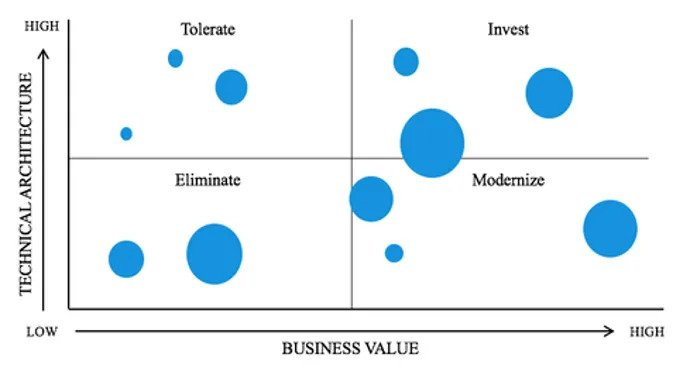
\includegraphics[width=12cm]{businessvalue}
\caption{Visuale representatie van businesswaarde voor mainframeapplicaties \autocite{Marble2017}}
\end{figure}



\subsection{\IfLanguageName{dutch}{Workloads migreren naar de cloud - Microservices}{Migrating workloads to the cloud - Microservices}}
\label{sec:Workloads migreren naar de cloud}

Een service is het ophalen of publiceren van data aan een remote systeem \autocite{Linthicum2016}. Volgens \textcite{Linthicum2016} is een voorbeeld van een service het proces om een risicoanalyse te berekenen bij een financiële transactie. Dat is de fundamentele werking achter een service-oriented architecture (SOA). Microservices is echter ook een architectuur, maar wordt volgens \textcite{Linthicum2016} vaak verward met een SOA. Er is natuurlijk wel een bepaalde overlap in de twee technologieën. Het ontwerppatroon dat erachter zit werkt door applicaties die bestaan uit kleine processen die met elkaar communiceren door het gebruik van application programming interfaces (API). De bedoeling bij service-oriented computing is dat applicaties worden gereduceerd tot enkel het functionele en die dan een set aan services aanbieden aan andere applicaties of de applicatie zelf. Het idee hierachter is het hergebruiken van functionaliteit \autocite{Linthicum2016}. 

Het gebruik van containers speelt bij microservices een grote rol. Met containers is het mogelijk om bestaande applicaties te gaan bundelen en de complexiteit te verlagen. Containers zorgen ervoor dat de applicaties niet meer afhankelijk zijn van hun onderliggende infrastructuurservices. Hierdoor is het mogelijk de toegang tot de opslag en resources los te koppelen van de applicaties en maakt dit de applicaties minder statisch \autocite{Linthicum2016a}. Microservices zijn net zo onafhankelijk en losgekoppeld. Het zijn geïsoleerde componenten die individueel kunnen gebruikt worden zonder effect op andere componenten. Het gebruik van Linux en/of Docker containers verzekeren dat services in dezelfde omgeving kunnen draaien in dezelfde omgeving \autocite{Bucchiarone2018}.

Volgens het rapport van \textcite{Bucchiarone2018} waarin de ervaring wordt beschreven van een migratie van een monolithisch systeem zoals mainframe naar Microservices, zal de mainframe voor lange tijd nog verbonden zijn aan de Microservice-technologie. Echter zal het mogelijk zijn om uiteindelijk de functionaliteiten van de mainframe te implementeren als nieuwe services. Dit zal resulteren in het definitief ontkoppelen van de mainframe \autocite{Bucchiarone2018}. 


\subsection{\IfLanguageName{dutch}{Workloads migreren naar de cloud - Amazon Web Services (AWS)}{Migrating workloads to the cloud - Amazon Web Services (AWS)}}
\label{sec:Workloads migreren naar de cloud}

Amazon Web Services is een cloudplatform van Amazon. AWS biedt organizaties middelen als rekenkracht, databankopslag en informatieleveringsdiensten. Het cloudplatform van Amazon is gelanceerd in 2006 en is gebaseerd op de infrastructuur waar Amazon.com op draait. Daarnaast zijn zij de eerste die pay-as-you-go cloud computing model aanbieden. Dit wil zeggen dat de infrastructuur geschaald wordt aan de hand van de opslag en rekenkracht noden van de klant \autocite{Gillis2020}.

\subsubsection{\IfLanguageName{dutch}{AWS Mainframe Modernization Service}{AWS Mainframe Modernization Service}}
\label{sec:AWS Mainframe Modernization Service }

Op 17 december 2021 vond er een event plaats waar de AWS Mainframe Modernization Service is geïntroduceerd. De principal product manager bij AWS is \textcite{Valence2021}  en daarnaast was hij ook de spreker op dit event. Volgens hem staan veel bedrijven voor grote uitdagingen met hun mainframeplatform. Veel organizaties komen met de vraag hoe zij hun assets van op hun mainframearchitectuur kunnen migreren naar AWS. Hij kaart volgende problemen met het mainframeplatform aan: 
 \begin{itemize}
    \item Complexe afhankelijkheden
    \item Beperkte en trage innovatie
    \item Oplopende kosten
    \item Gebrek aan skills
    \item Ontoegankelijke data
    \item Strikte afhankelijkheden
    \item Gelimiteerde capaciteit
    \item Outdated interfaces 
    \item Legacy componenten
    \item Ongedocumenteerde applicaties 
    \item Langdurige investering 
\end{itemize}

De voornaamste redenen volgens \textcite{Valence2021} die bedrijven aankaarten te willen migreren zijn om hun kosten te reduceren, risico's te verminderen en hun flexibiliteit te verhogen. Flexbiliteit in de zin dat organisaties zo snel mogelijk willen kunnen beantwoorden aan externe veranderingen zoals de vraag van de klant of de hoeveelheid dataverwerking. Daarnaast willen organisaties de kosten die de mainframe met zich meebrengt omruilen voor investeringen in nieuwe innovaties. Deze vereisten zijn de dreefveer achter de migratieplannen maar tegelijk willen ze de RAS-factoren (reliabilty, availability, serviceability) die de mainframe biedt ook behouden bij een migratie naar een cloudomgeving. AWS Mainframe Modernization Service is volgens \textcite{Valence2021} een uniek platform voor het migreren, moderniseren en uitvoeren van mainframeapplicaties. Deze service is in staat om mainframeapplicaties uit te voeren en te beheren. Bij het migreren naar het AWS-platform zijn vier fases betrokken waaronder analyseren, ontwikkelen, deployen en beheren. Zoals aangegeven bij vorige strategieën, waaronder die van \textcite{Marble2017}, is analyseren van de workloads een belangrijk onderdeel. Het is belangrijk om een kijk te nemen naar alle afhankelijkheden, businesswaarde en complexiteit van elke applicatie om te kunnen bepalen in welke volgorde de migratie wordt uitgevoerd. 

De tweede fase is de ontwikkelfase. Dit is de fase waar de migratie gebeurd, zoals het hercompileren, herformatteren van data of conversies om te voldoen aan de artefacten van de nieuwe doelapplicatie. Bij de deployfase vertelt \textcite{Valence2021} dat hier de unieke mogelijkheden verborgen zitten aan de AWS Mainframe Modernization Service. Hier wordt namelijk een runtime omgeving opgezet voor de mainframeapplicaties. De bedoeling is dat een organisatie een runtime omgeving volledig zelf kan creëren en hun applicaties hierop kunnen deployen. 

Via AWS Blu Age is het mogelijk om aan automatische code refactoring te doen. Hierbij is het mogelijk gemaakt door AWS om legacy applicaties die werden geschreven in COBOL of PL/1 te refacteren naar Java of batchscripts. De AWS Blu Age is een ketting van verschillende stappen binnen het moderniseren. Er zal aan reverse-engineering en forward-engineering gedaan worden om runtime instanties te kunnen verkrijgen van applicaties geschreven in een mainframespecifieke programmeertaal. Volgens \textcite{Valence2021} is het de bedoeling van de AWS Blu Age Toolchain om een moderne Angular front-end webservice te krijgen die Java services aanspreekt via een REST API op basis van de mainframe legacy.  

Bij het opzetten van een moderniseringsproject voor het migreren van mainframe naar AWS volgt AWS een plan dat gebaseerd is op het Migration Accelaration Program (MAP). Dit programma is afkomstig van gedistribueerde systemen en is een waardig cloudmigratieprogramma. Het is gebaseerd op duizende best practices op vlak van een migratie. AWS heeft dit programma aangepast zodat het specifiek inzetbaar is voor een migratie van een mainframeplatform. Volgens \textcite{Valence2021} geeft dit programma een garantie op het slagen van een migratieproject. Het MAP steunt op 6 pilaren waaronder:
 \begin{itemize}
    \item Migratiemethodologieën
    \item AWS tools
    \item AWS partners
    \item AWS investeringen
    \item AWS trainingen
    \item AWS professionele services
\end{itemize}

AWS raadt sterk aan om bij een migratieproject, dat gebruik maakt van de AWS Mainframe Modernization Service, een expert of meerdere experten aan te werven die kennis hebben van de toolchains die AWS aanbiedt. Volgens \textcite{Valence2021} is het van essentieel belang dat organisaties hulp in roepen van specialisten om het succes van een migratieproject te garanderen. 

\subsubsection{\IfLanguageName{dutch}{Een praktische uitwerking: het uitvoeren van een COBOL applicatie op AWS Lambda}{A practical implementation: running a COBOL application on AWS Lambda}}
\label{sec: Een praktische uitwerking: uitvoeren  van COBOL applicatie op AWS Lambda}

Met deze praktische uitwerking willen we aantonen hoe eenvoudig of complex het is om gebruik te maken van de functies die AWS biedt om aan migratie te doen.

Via AWS Lambda is het mogelijk om via hosted services aan serverless computing te doen op AWS. Volgens \textcite{Sbarski2017} is serverless computing een bevestiging van hoe een intelligente combinatie van services een vermindering kan teweegbrengen op vlak van de tijd die ontwikkeling met zich meebrengt en de kosten. Deze nieuwe architectuur laat de kosten die serversoftware of mainframesoftware met zich meebrengen verdwijnen en het biedt de flexibiliteit om snel te ontwikkelen, deployen en applicaties te beheren \autocite{Sbarski2017}. Lambda kan code uitvoeren op een extreem parallelle manier als response op een event. Zonder behulp van servers is het mogelijk om via Lambda code te gaan uitvoeren. Het is niet meer nodig om na te denken over het intalleren van software, het deployen van containers of andere details \autocite{Sbarski2017}. AWS zorgt ervoor dat hun Elastic Compute Cloud (EC2) servers de code uitvoert met in het achterhoofd zaken te voorzien als schaalbaarheid en beschikbaarheid zodat de ontwikkelaar hier niet meer over hoeft na te denken. Serverless architectuur verwijst eigenlijk naar een architectuur waar het niet meer noodzakelijk is om een directe connectie te hebben met een mainframe of server. Als gevolg hiervan kunnen ontwikkelaars zich enkel focussen op het kwalitatief schrijven van code. Hieronder bevinden zich de vijf principes waar een serverless architectuur op steunt:
 \begin{itemize}
    \item Het gebruik van een compute service om code uit te voeren zonder servers of mainframes
    \item Het schrijven van fucnties met één enkel doel
    \item Event-driven pipelines
    \item Het bouwen van krachtigere front-ends
    \item het gebruik van third-patry services
\end{itemize}

AWS Lambda is een compute service dat code uitvoert op de Amazon Web Services infrastructuur. De broncode van applicaties wordt uitgepakt en gedeployed op een geïsoleerde container met zijn eigen gealloceerd geheugen en central processing unit. De combinatie van code, configuraties en afhankelijkheden staan bekend onder een Lambda functie. Lambda ondersteunt daarnaast push en pull events en integreert een groot aantal AWS services. 
\begin{figure}[h]
    \centering
    \begin{subfigure}{0.45\textwidth}
        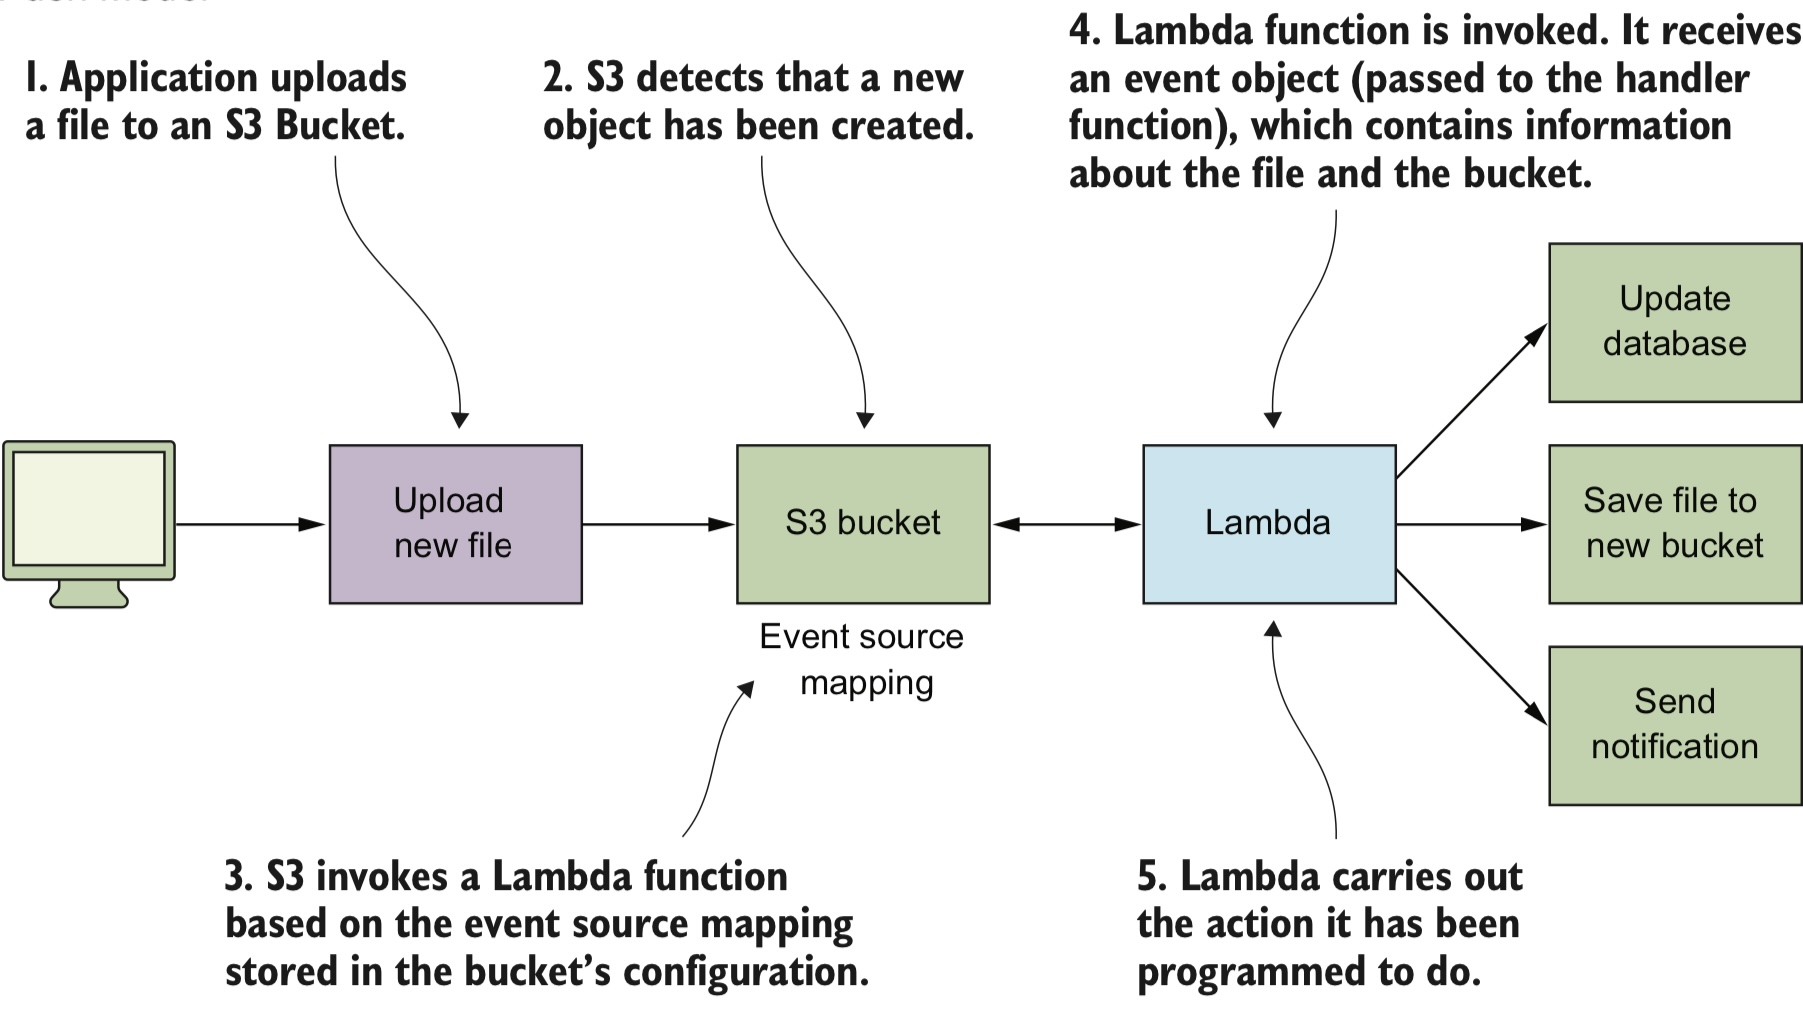
\includegraphics[width=\textwidth]{push_model}
        \caption{Voorbeeld van het push model \autocite{Sbarski2017}}
    \end{subfigure}
    \hfill
    \begin{subfigure}{0.45\textwidth}
        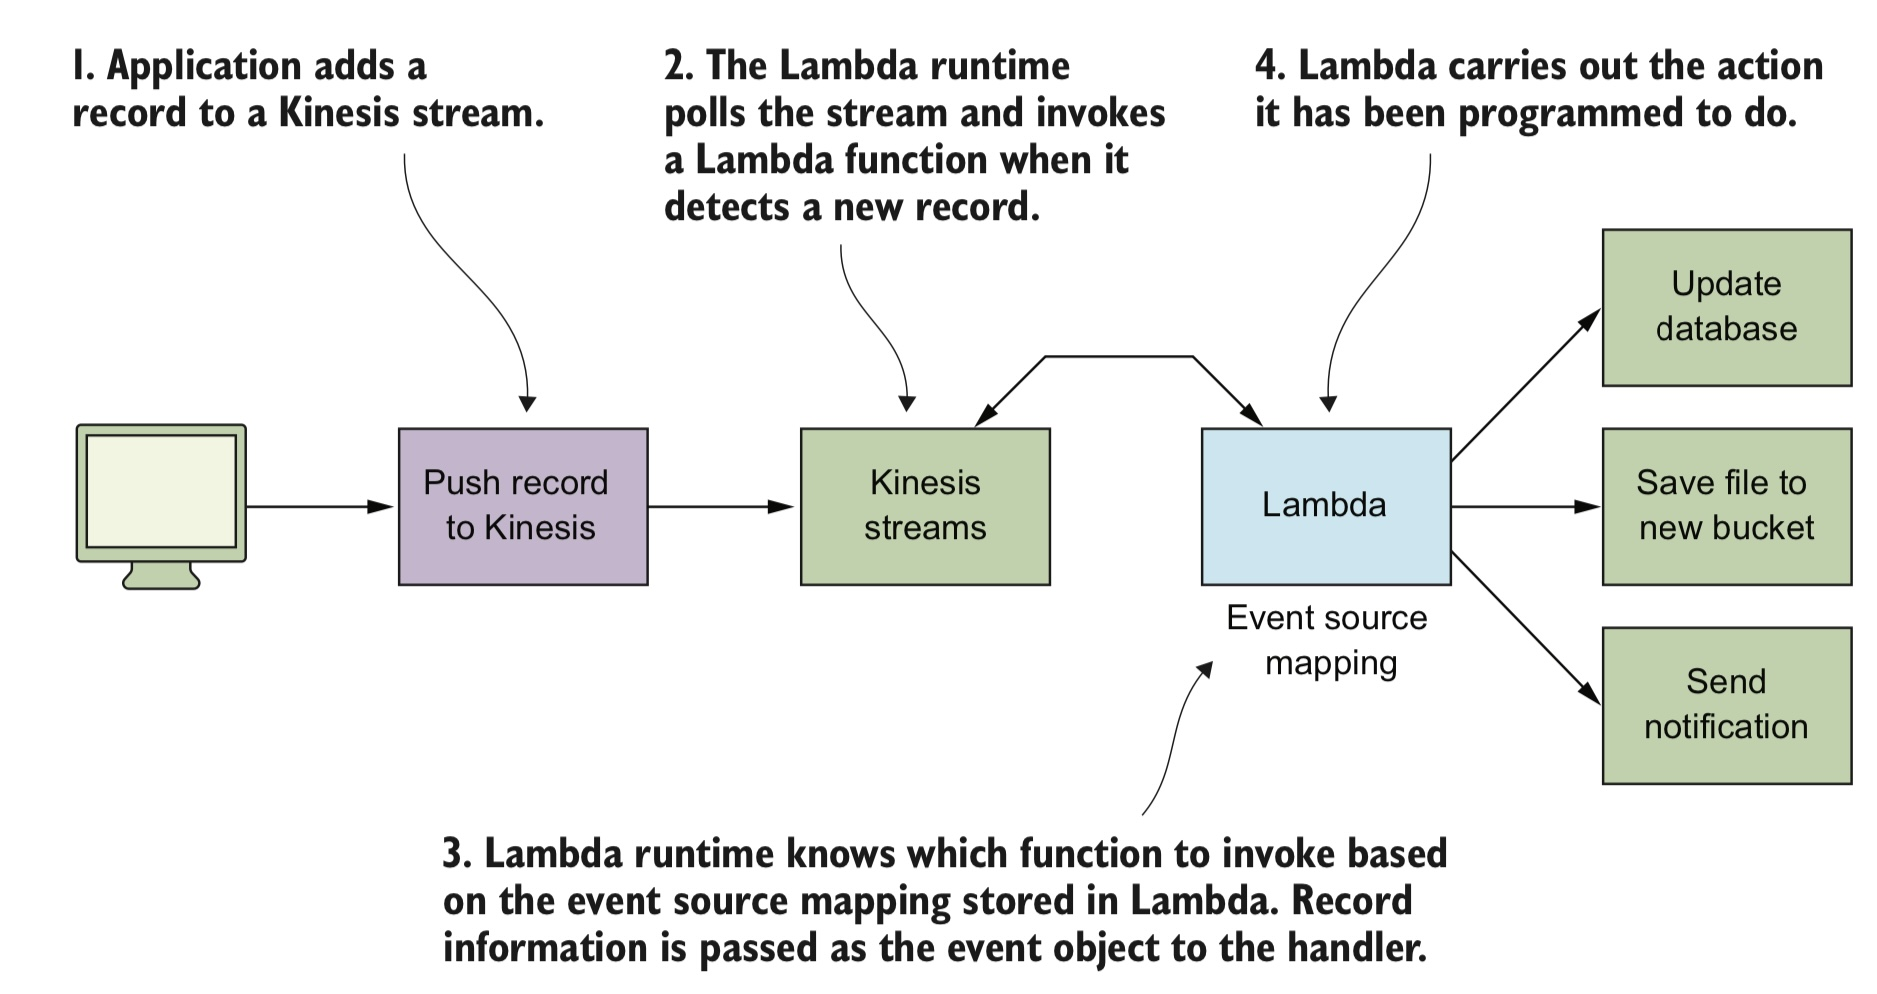
\includegraphics[width=\textwidth]{pull_model}
        \caption{Voorbeeld van het pull model \autocite{Sbarski2017}}
    \end{subfigure}
\end{figure}

Als praktische uitwerking is in het onderzoek is met behulp van een AWS Lambda functie een kleine COBOL applicatie uitgevoerd op het AWS platform. Deze uitwerking werd gedaan met behulp van het stappenplan van \textcite{Paika2020}. Volgens \textcite{Paika2020} is dit een ideale manier om aan te tonen hoe een AWS Lambda functie in zijn werk gaat. Eerst en vooral werd de COBOL code voor een simpel ``Hello World `` programma lokaal compileerd en uitgevoerd in een terminal zoals hieronder weergegeven. De compiler die hier werd gebruikt is GnuCOBOL.  
    \begin{figure}[h]
        \centering
        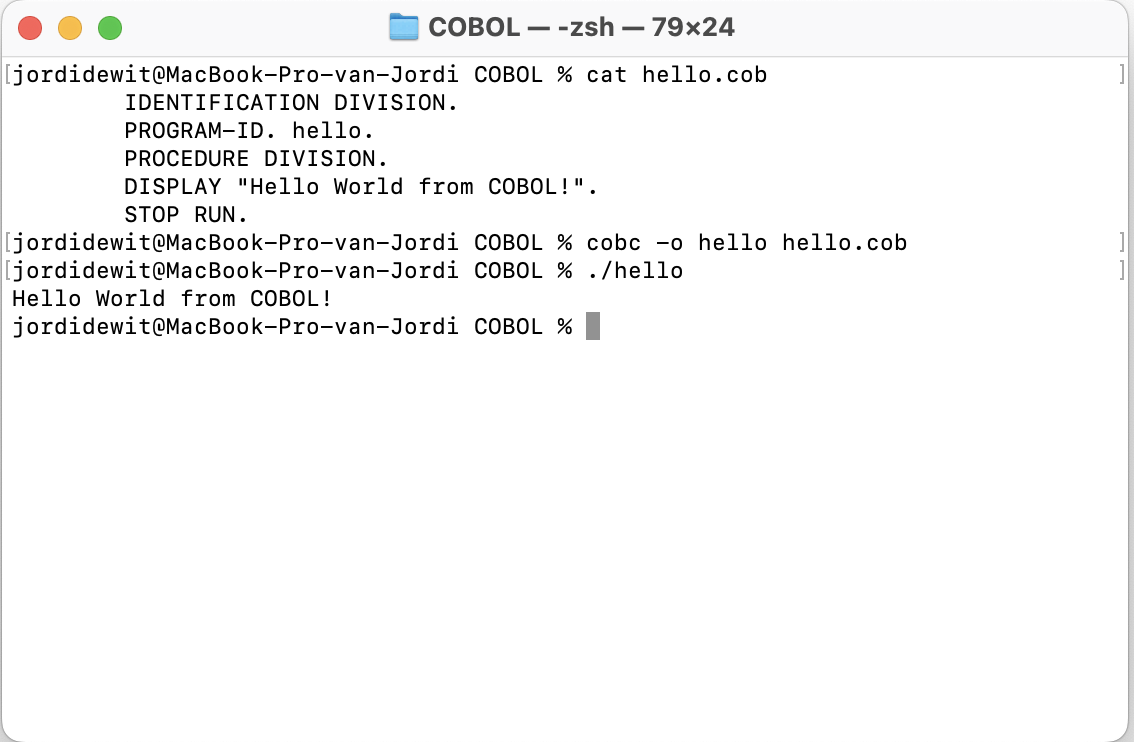
\includegraphics[width=10cm]{gnucobol}
        \caption{Het lokaal uitvoeren van een COBOL programma met GnuCOBOL.}
     \end{figure}
 
 Vervolgens was het de bedoeling volgens het stappenplan van \textcite{Paika2020} dat we een runtimeomgeving opzetten door gebruik te maken van een AWS Lambda functie. Dit kon bereikt worden via de Amazon Linux 2 AWS Lambda executieomgeving. Hiervoor was het nodig om een bootstrap script te creëren om een uitvoering te voorzien zodra de Lambda functie wordt geïnitialiseerd. Amazon Linux 2 kon worden gevirtualiseerd in een docker file. Hier was het mogelijk om het COBOL programma te compileren omdat Amazon Linux 2 ook gebruik maakt van GnuCOBOL. Op onderstaande afbeelding is te zien hoe dit proces in zijn werk ging. 
 
 WORDT VERVOLGD...
 
 \newpage
 
 \section{\IfLanguageName{dutch}{De resultaten van de bevragingen}{The results of the survey}}
 \label{sec:De resultaten van de bevraging}
 
 Om in dit onderzoek ook een beeld te kunnen schetsen omtrent de hedendaagse meningen rond het gebrek aan expertise, migratieplannen en interesse voor mainframe bij studenten en IT-professionals werd een enquête opgesteld. Deze enquête heeft volgende resultaten opgeleverd.
 
  \subsection{\IfLanguageName{dutch}{De resultaten van de bevragingen voor bedrijven}{The results of the survey for organizations}}
 \label{sec:De resultaten van de bevraging}

Vijf bedrijven hebben antwoorden gegeven op mijn enquête waaronder: 
 \begin{itemize}
    \item KBC
    \item Colruyt Group
    \item Nationaal Vebond van Socialistische Mutualiteiten
    \item SD Worx
    \item Volvo Group
\end{itemize}

De resultaten zijn opgedeeld per vraag. 

 \subsubsection{\IfLanguageName{dutch}{In welke sector is het bedrijf actief?}{In which sector is the organization active?}}
\label{sec:In welke sector is het bedrijf actief}

 \begin{figure}[h]
    \centering
    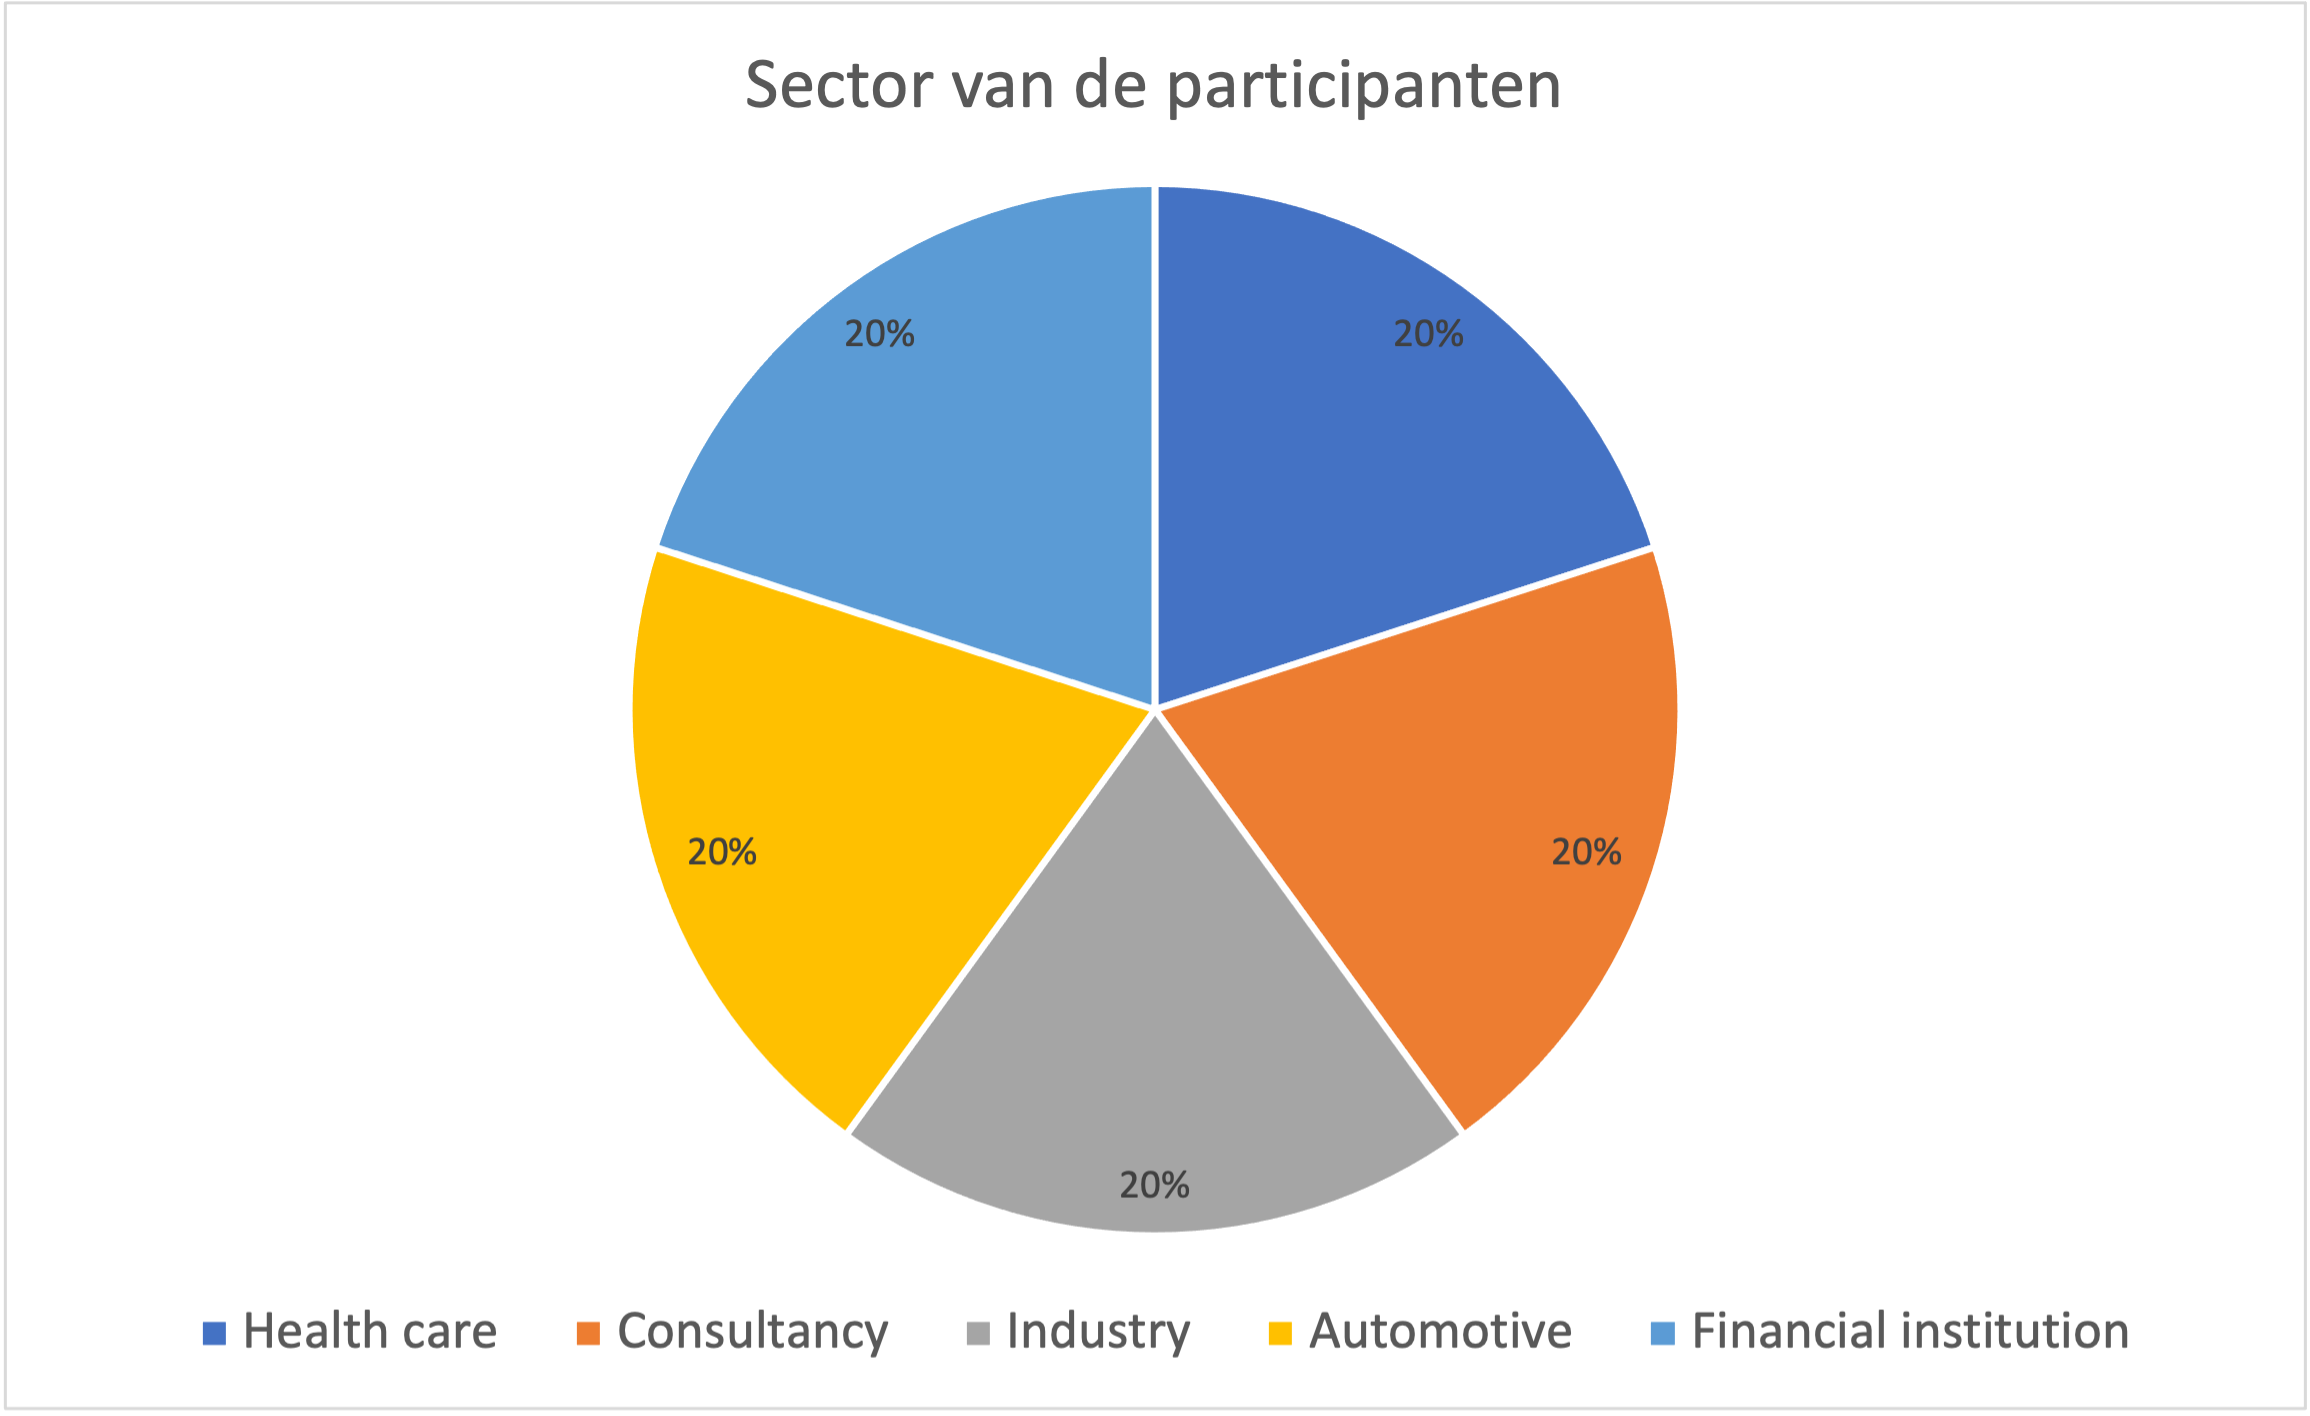
\includegraphics[width=12cm]{sector_grafiek}
    \caption{De verdeling van de deelnemende organisaties per sector.}
\end{figure}

Uit bovenstaande grafiek is af te leiden dat de participanten die we classificeren als een bedrijf gelijk verdeeld waren. Uit elke sector heeft juist één bedrijf deelgenomen aan de bevraging rond het onderzoek. Daarnaast heeft elk bedrijf uit deze grafiek een mainframe in gebruik. 

\newpage

 \subsubsection{\IfLanguageName{dutch}{Wat is het aantal van werknemers die werk leveren dat te maken heeft met het ontwikkelen, onderhouden of beheren van een mainframe?}{What is the number of employees who develop, maintain or manage a mainframe?}}
\label{sec:Wat is het aantal van werknemers die werk leveren dat te maken heeft met het ontwikkelen, onderhouden of beheren van een mainframe?}

 \begin{figure}[h]
    \centering
    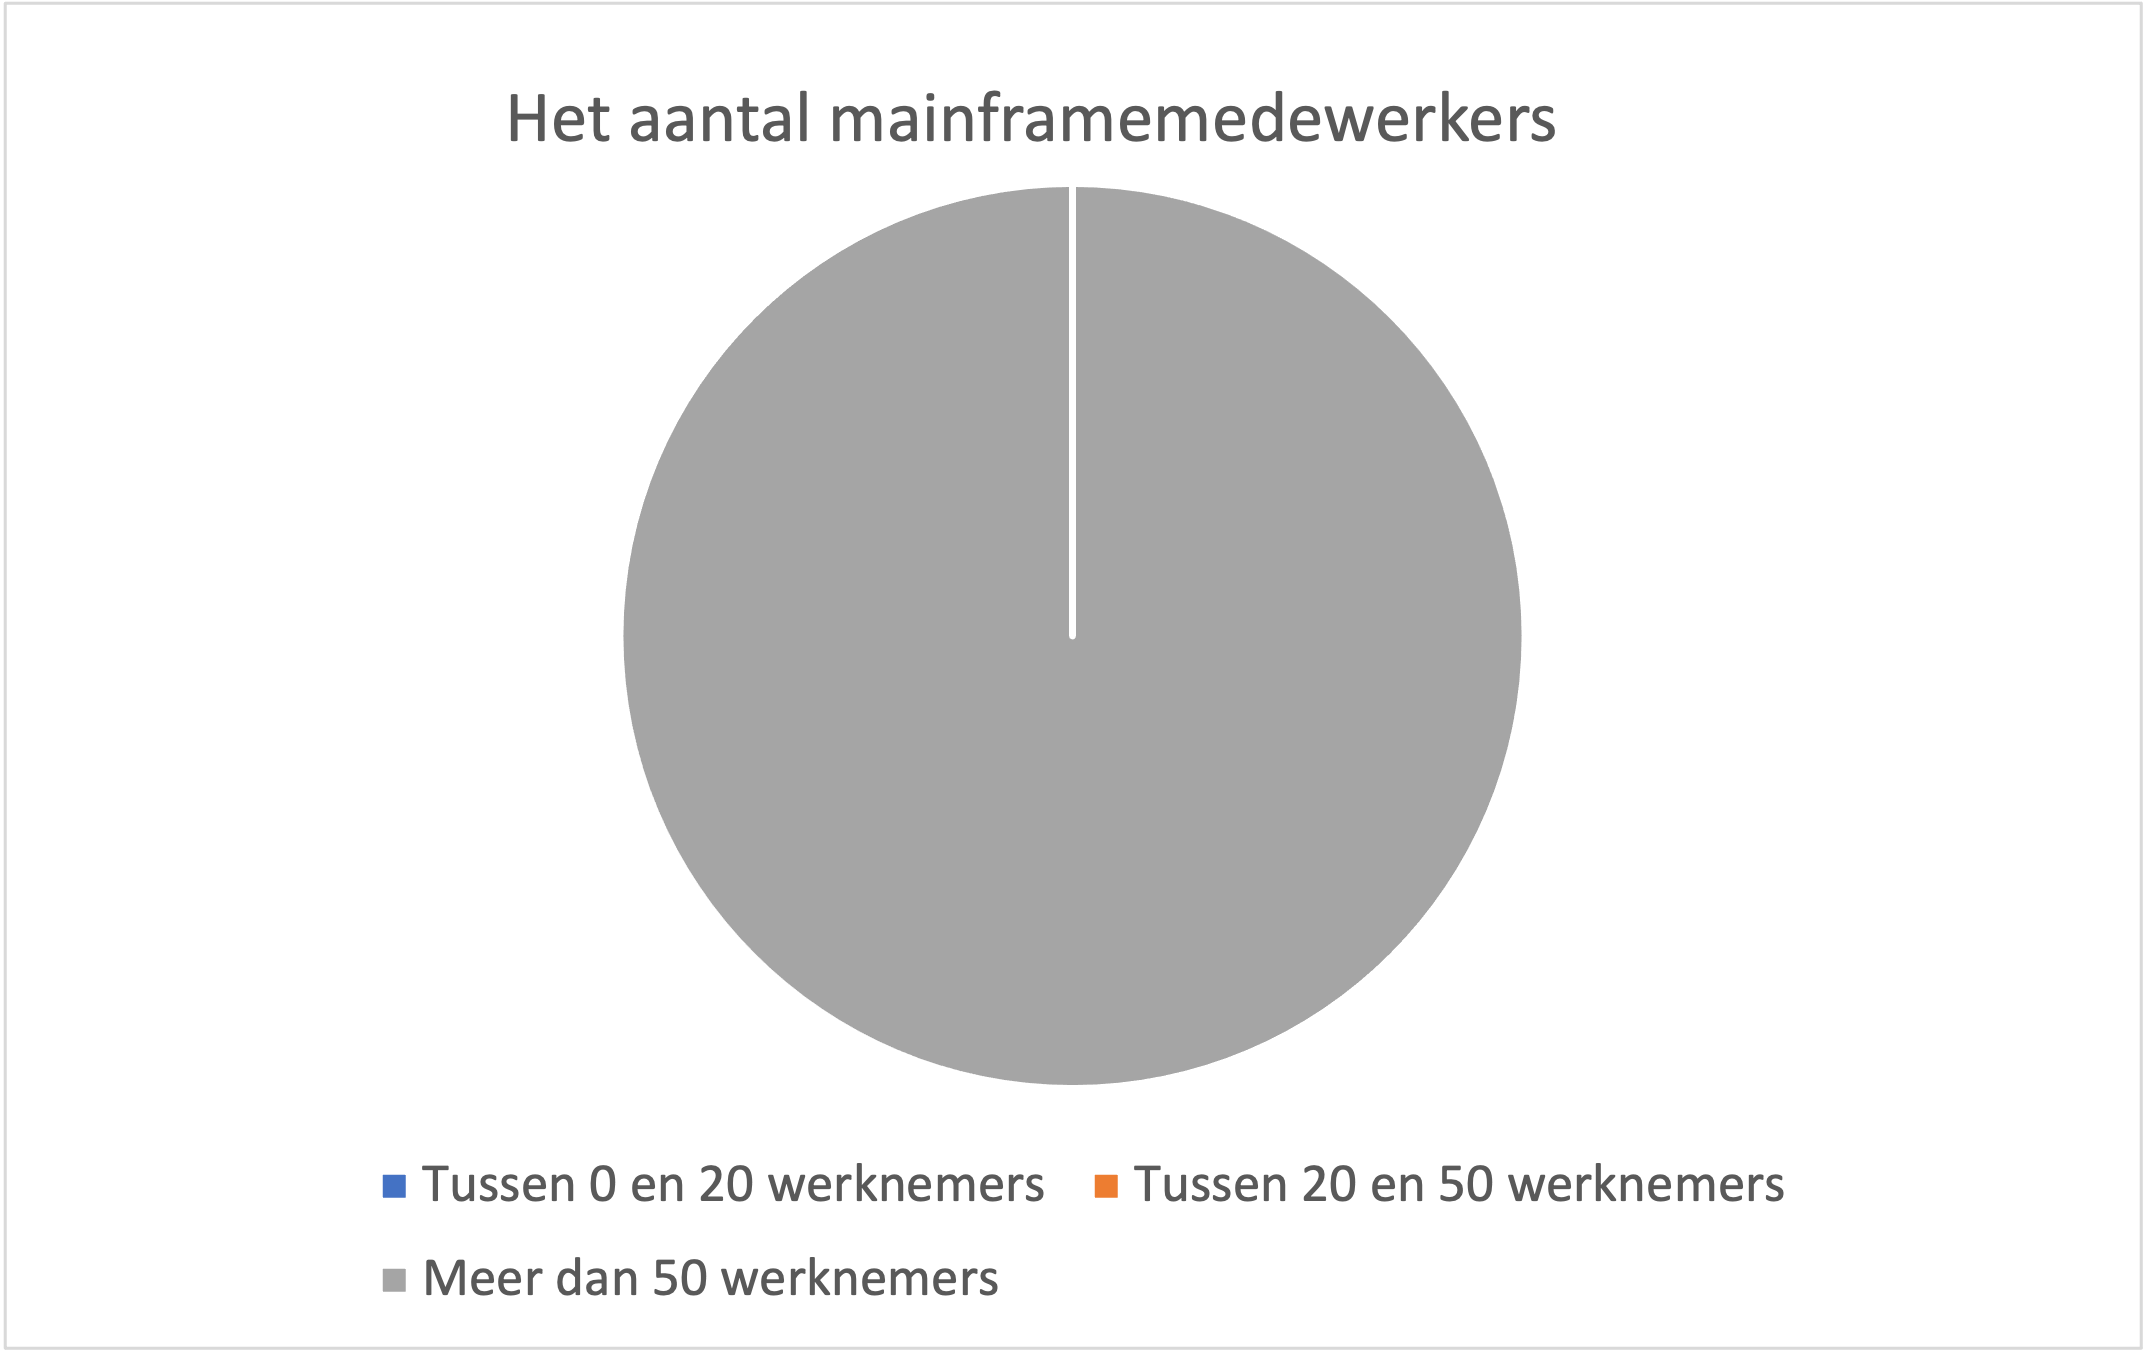
\includegraphics[width=12cm]{werknemers_grafiek}
    \caption{De grafiek met het aantal werknemers dat op mainframe werkt.}
\end{figure}

Elk van de bevraagde bedrijven heeft meer dan 50 mensen in dienst die werken op mainframe. Dit omvat het ontwikkelen van applicaties, het onderhouden van applicaties of beheren van het systeem. Hieruit kan geconcludeerd worden hoe hoog de nood is aan mainframewerkkrachten. Het is echter een groot deel van een IT-afdeling binnen de deelnemende organisaties.

 \subsubsection{\IfLanguageName{dutch}{Wat is de gemiddelde leeftijd van het mainframepersoneel?}{What is the average age of the mainframe staff?}}
\label{sec:Wat is de gemiddelde leeftijd van het mainframepersoneel?}

\begin{figure}[h]
    \centering
    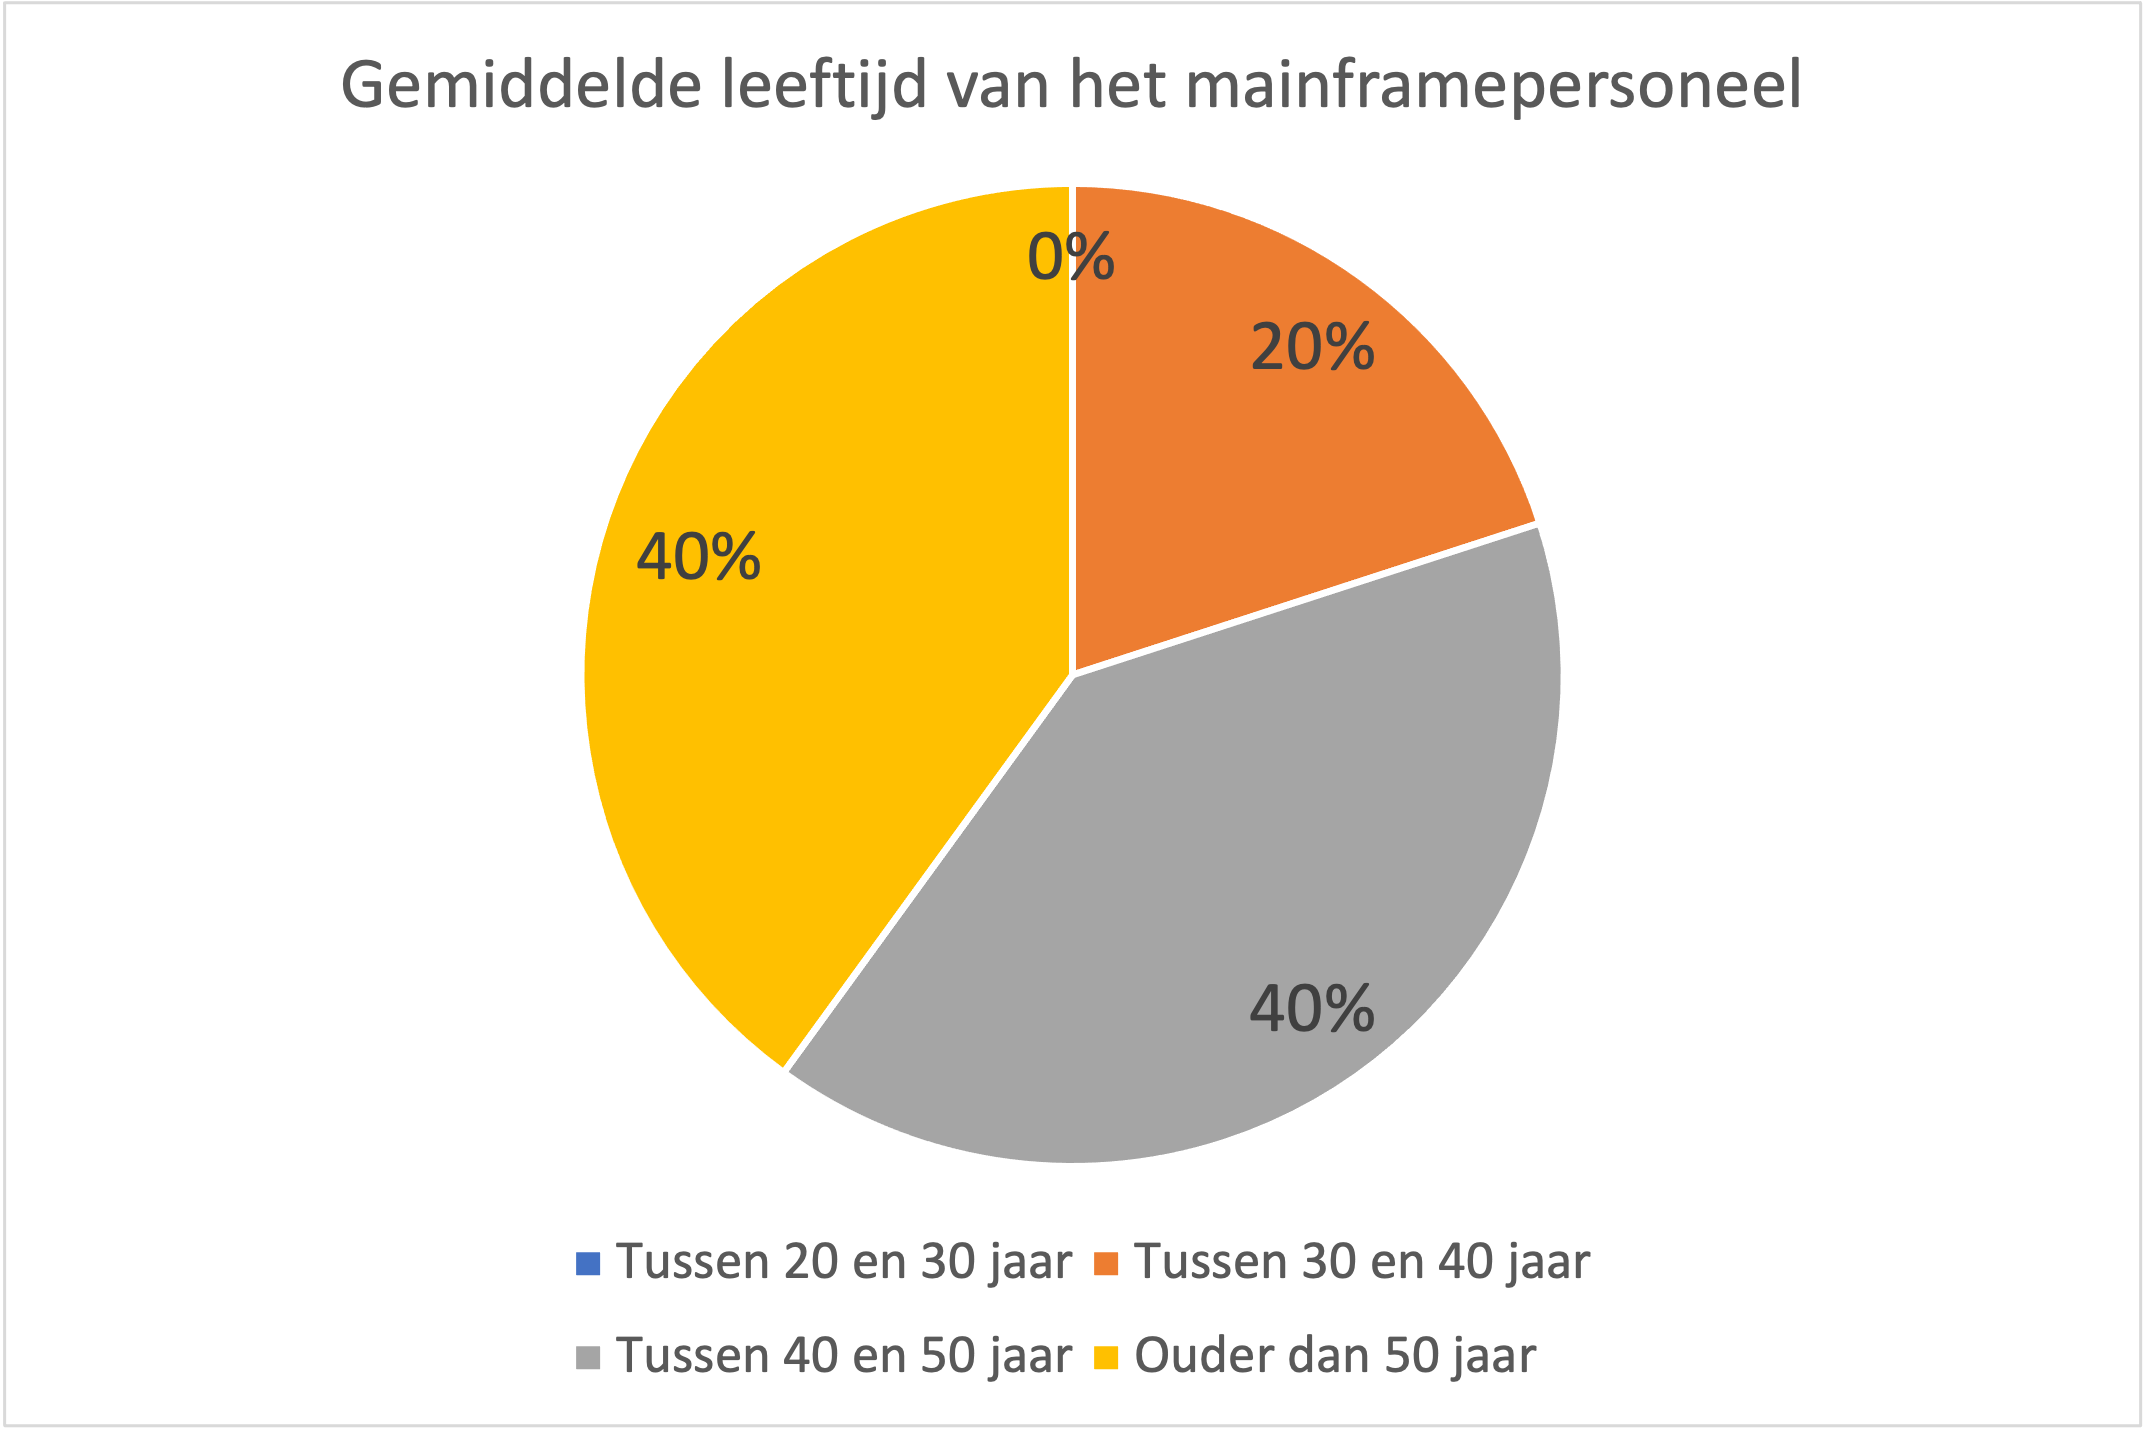
\includegraphics[width=12cm]{gemiddelde_leeftijd_grafiek}
    \caption{De grafiek met de gemiddelde leeftijd van het mainframepersoneel.}
\end{figure}


De gemiddelde leeftijd binnen de deelnemende organisaties ligt opmerkelijk hoog. Twee op vijf bedrijven geeft aan dat hun mainframepersoneel een gemiddelde leeftijd heeft die hoger ligt dan 50 jaar. Slechts één bedrijf geeft aan dat hun mainframepersoneel een gemiddelde leeftijd heeft tussen 30 en 40 jaar ligt. De andere bedrijven geven een leeftijd aan tussen 40 en 50 jaar. 

WORDT VERVOLGD MET RESULTATEN... 




